\documentclass[a4paper,margin,line]{resume}
\usepackage[defblank]{paralist}
\usepackage{pdfpages}
\usepackage{blfootnote}
\usepackage{anysize}
\usepackage[pdftex]{hyperref}
\hypersetup{pdftitle={Russell Harmon's Resume}}
\hypersetup{pdfauthor={Russell Harmon}}
\hypersetup{pdfborder={0 0 0}}
\hypersetup{unicode=true}
\marginsize{2.5mm}{35mm}{2.5mm}{1mm}
\setdefaultitem{\tiny \textbullet}{}{}{}{}{}
\setdefaultleftmargin{0em}{}{}{}{}{}
\begin{document}
\name{\Large Russell E. Harmon}
\begin{resume}

\section{\mysidestyle Contact \\ Information}\vspace{2mm}
	\begin{asparablank}
		\item Rochester Institute of Technology \hfill 2710 Avenue J NW
		\item 39 Nathaniel Rochester Hall \hfill Winter Haven, FL 33881
		\item Rochester, NY 14623 \hfill \href{mailto:russ@eatnumber1.com}{russ@eatnumber1.com}
		\item (863) 514-7014 \hfill
		\href{http://blog.eatnumber1.com}{blog.eatnumber1.com}
	\end{asparablank}

\section{\mysidestyle Objective}
	Obtain a three to six month co-op/internship that will serve to broaden my
	horizons in the field of Computer Science.

\section{\mysidestyle Education}
	\begin{compactdesc}
		\item[Rochester Institute of Technology] \hfill {\footnotesize 2006 - Present}
		\begin{compactitem}
			\item {\small Major: Bachelors/Masters in Computer Science}
			\item {\small Minor: Music}
			\item {\small Expected graduation: 2012}
		\end{compactitem}
		\item[Herbert H. Lehman High School] - College Prep Program \hfill
		{\footnotesize 2002 - 2006}
		\item[Lehman College] - Course work in Q-Basic (age 12) \hfill
		{\footnotesize September 2000 - December 2000}
	\end{compactdesc}

\section{\mysidestyle Experience}
	\begin{compactdesc}
		\item[SafeNet Inc] - Belcamp, MD \hfill {\small June 2008 - Present}
		\\* Engineering Intern \hfill {\footnotesize
		\url{http://www.safenet-inc.com}}
		\begin{compactitem}
			\item {\small Working as a developer on a team of 7 on SMCII (the
			SafeNet Management Console)}
			\item {\small Java development with JBoss, Hibernate and JSF}
		\end{compactitem}
		\item[New York City Department of Education] - Bronx, NY \hfill
		{\small September 2002 - June 2006}
		\\* IT Specialist \hfill {\footnotesize \url{http://schools.nyc.gov}}
		\begin{compactitem}
			\item {\small Setup and maintain computer systems throughout Lehman
			High School}
			\item {\small Repair, and maintain the network}
			\item {\small Diagnose and eliminate viruses and malware on the
			school's network and computer systems}
			\item {\small Audit the network for malicious activity}
		\end{compactitem}

		\item[New York Sailing \& Yacht Club] - Bronx, NY \hfill {\small
		2001-2005}
		\\* Launch Operator \hfill {\footnotesize \url{http://www.startsailing.com}}
		\begin{compactitem}
			\item {\small Taxi patrons to their boats moored in the harbor}
			\item {\small Small craft operation - experienced in motor and sail
			boats}
		\end{compactitem}

		\item[City Island Computer Services] - Bronx, NY \hfill {\small
		1998-1999}
		\\* Apprentice (age 10)
	\end{compactdesc}

% HACK: Each toplevel \item here requires an escaped whitespace character in
% order to force the item to appear on it's own line (since the text of the item
% is the bullet, so the item has no text).
\section{\mysidestyle Technical Skills}
	\begin{compactdesc}
		\item[Languages] \ 
		\small
		\begin{compactitem}
			\item Java
			\item C/C++
			\item bash/sh and other ksh derived shell scripting languages
			\item Python
		\end{compactitem}
		\normalsize
		\item[Operating Systems] \ 
		\small
		\begin{compactitem}
			\item Linux
			\item Solaris
		\end{compactitem}
		\normalsize
		\item[Hardware] \ 
		\small
		\begin{compactitem}
			\item PC troubleshooting and repair
			\item Networking
			\item Network Security
		\end{compactitem}
		\normalsize
	\end{compactdesc}

\section{\mysidestyle Honors \& Awards}
	\begin{asparablank}
		\item NYC Regional Robotics Award winner
		\begin{compactitem}
			\item {\small 27th place in the national competition}
		\end{compactitem}
		\item Honor Roll 2003-2005
		\item Visual Basic Programming Award for academic excellence 2005
		\item First Place Sailing Award 2000, 2002
	\end{asparablank}

\section{\mysidestyle Special Accomplishments}
	\begin{asparablank}
		\item At age 8, built my first computer. At age 12, attended my first
		programming class at Lehman College.
		\item Designed and implemented an encryption algorithm using a
		combination of transposition and substitution.
		\item Community Service - built a boat for needy children from the South
		Bronx.
	\end{asparablank}

\section{\mysidestyle Personal \\ Strengths}
	\begin{asparablank}
		\item Ingenuity
		\item Thinking Outside the Box
		\item Perseverance
		\item Motivated to Excel
	\end{asparablank}

\section{\mysidestyle Certifications}
	\begin{asparablank}
		\item Cisco Academy, with honors (terms 1 and 2)
		\item A+
		\item MOUS (Word)
	\end{asparablank}

\blfootnote{References available on request.}
\end{resume}
\pagebreak[4] % The 4 makes it a VERY INSISTENT requirement for a page break.
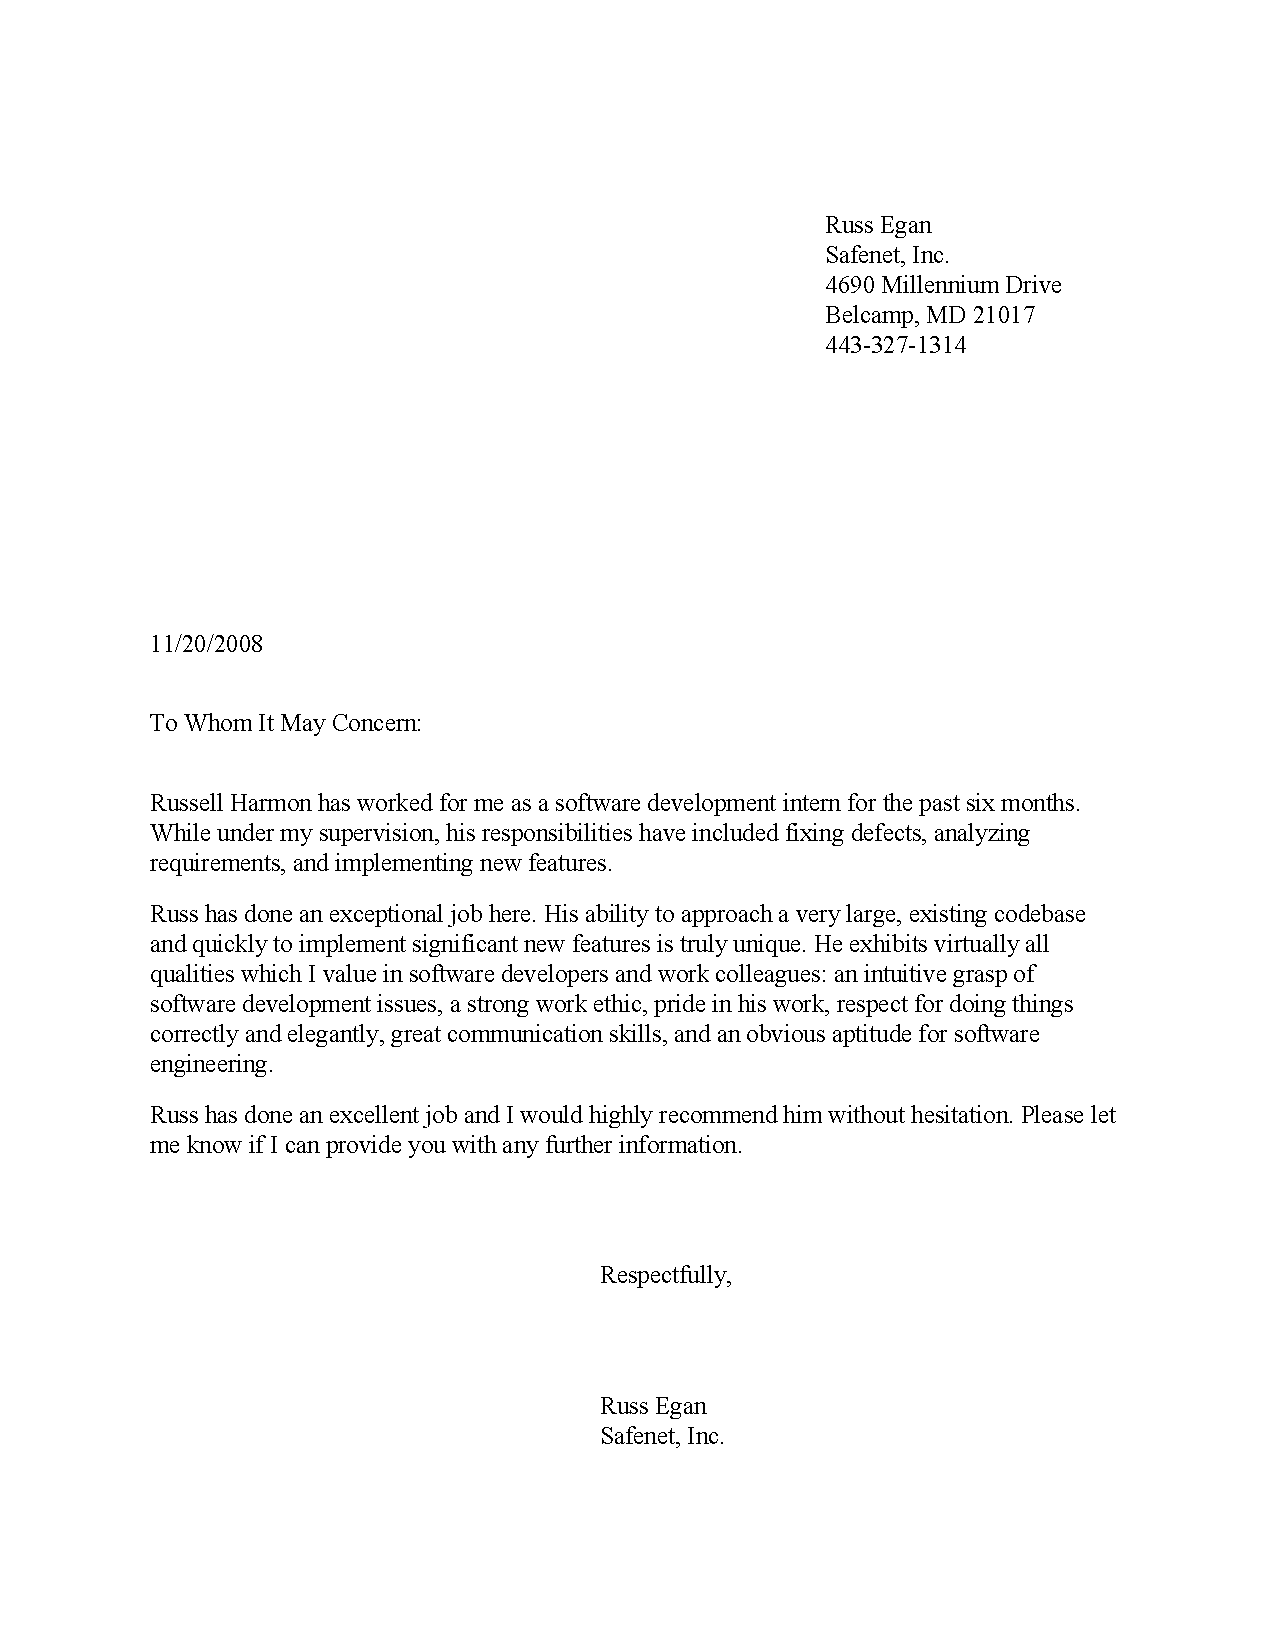
\includepdf[offset=-94 0,pages=1]{sfnt-recommendation}
\end{document}
